\subsection{Power}

Mobile devices employ dynamic voltage frequency scaling (DVFS),
  this results in power draw of the device being goverened by
  the operating frequency of the processor.
One can model the battery usage of the power draw at time $t$~\cite{zhang2010accurate, dong2011self} is

$$
P(t) = BatV(Brightness(t)) + GPUU(t) * GPUV(GPUF(t)) + sum_{i=1}^{N} CPUU_n(t) * CPUV_n(CPUF_n(t))
$$

with $N$ begin the number of CPU cores, $Brightness$ is the brightness of the LCD screen at time $t$, $BatV(br)$ is the power used for the specified brightness level, $GPUF(t)$ and $CPUF(t)$ are the operating frequencies at time $t$, and $GPUV(f)$ and $CPUV(f)$ are the power draws for the processors at the specified voltage, $GPUU(t)$ and $GPUU_n(t)$ are the processor utlization at time $t$.
Other terms, such as GPS, wireless, and other sensors, can be measured or modeled, but for this analysis we turn them off.

The issues with using a model are knowing the the power draw at the 
  frequency (which is not specified by the processor's manifacturer) and the method of reading
  the CPU and GPU counters is varies from device to device.
As a result, we use Qualcomm's Trepn tool~\cite{profilerqualcomm} to read the hardware
  counters.
Battery information consists of all power-consuming components, e.g., screen,
cpu, gpu, memory.
If the computation takes longer, more power is consumed by other components, such as the LCD screen.
Therfore, power is not only a measure of the load, but also the time it takes to perform a computation.

\begin{figure}[tp]
  \centering

  \begin{subfigure}[b]{0.5\textwidth}
          \centering
          
\includegraphics[width=0.6\textwidth]{data/legend.pdf}
  \end{subfigure}

  \begin{subfigure}[b]{0.24\textwidth}
      \centering
      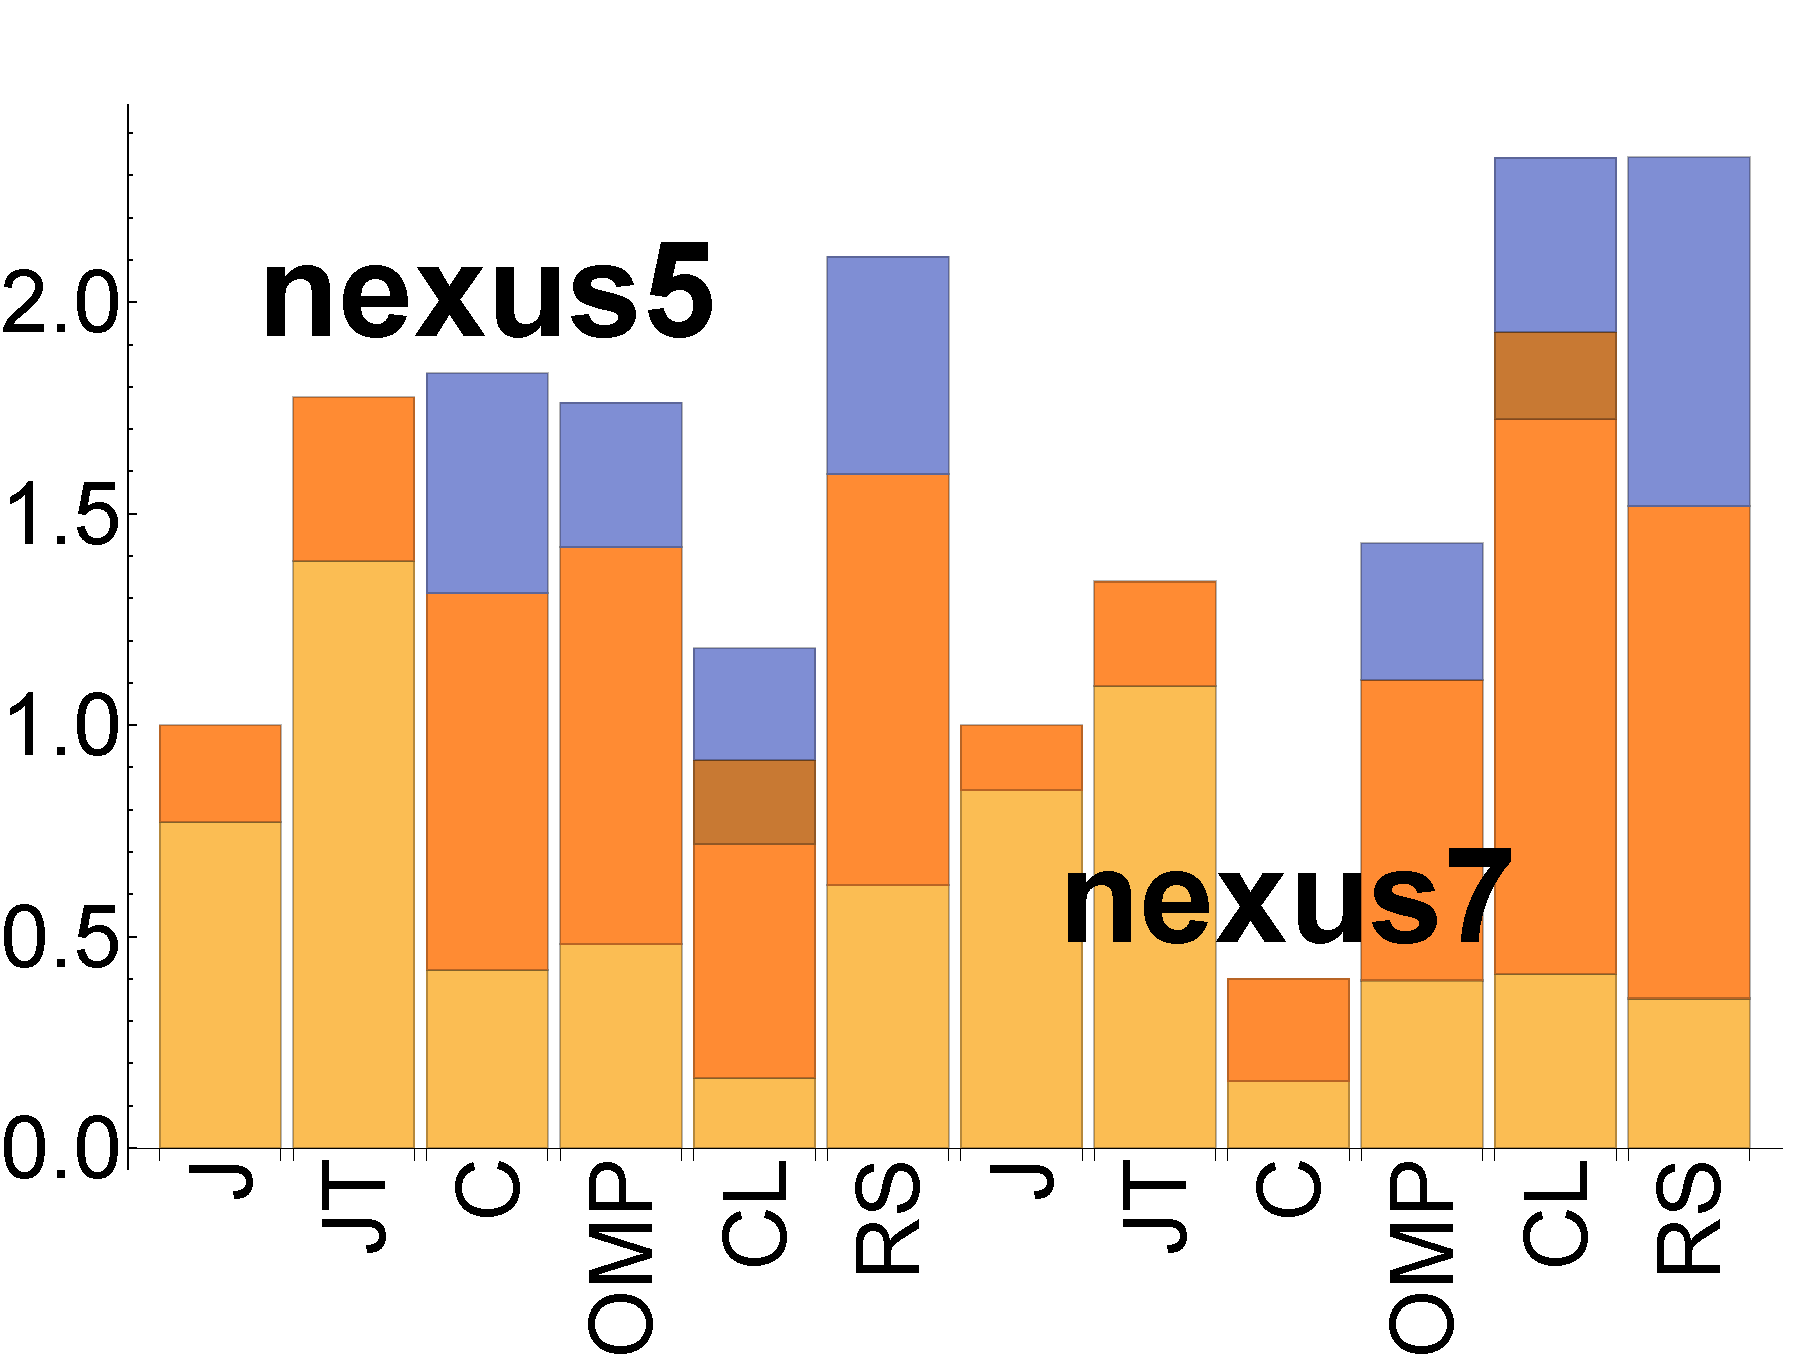
\includegraphics[width=\textwidth]{data/bbattery_vectoradd.pdf}
      \caption{VectorAdd}\label{fig:b_vectoradd}
  \end{subfigure}%

  \begin{subfigure}[b]{0.24\textwidth}
      \centering
      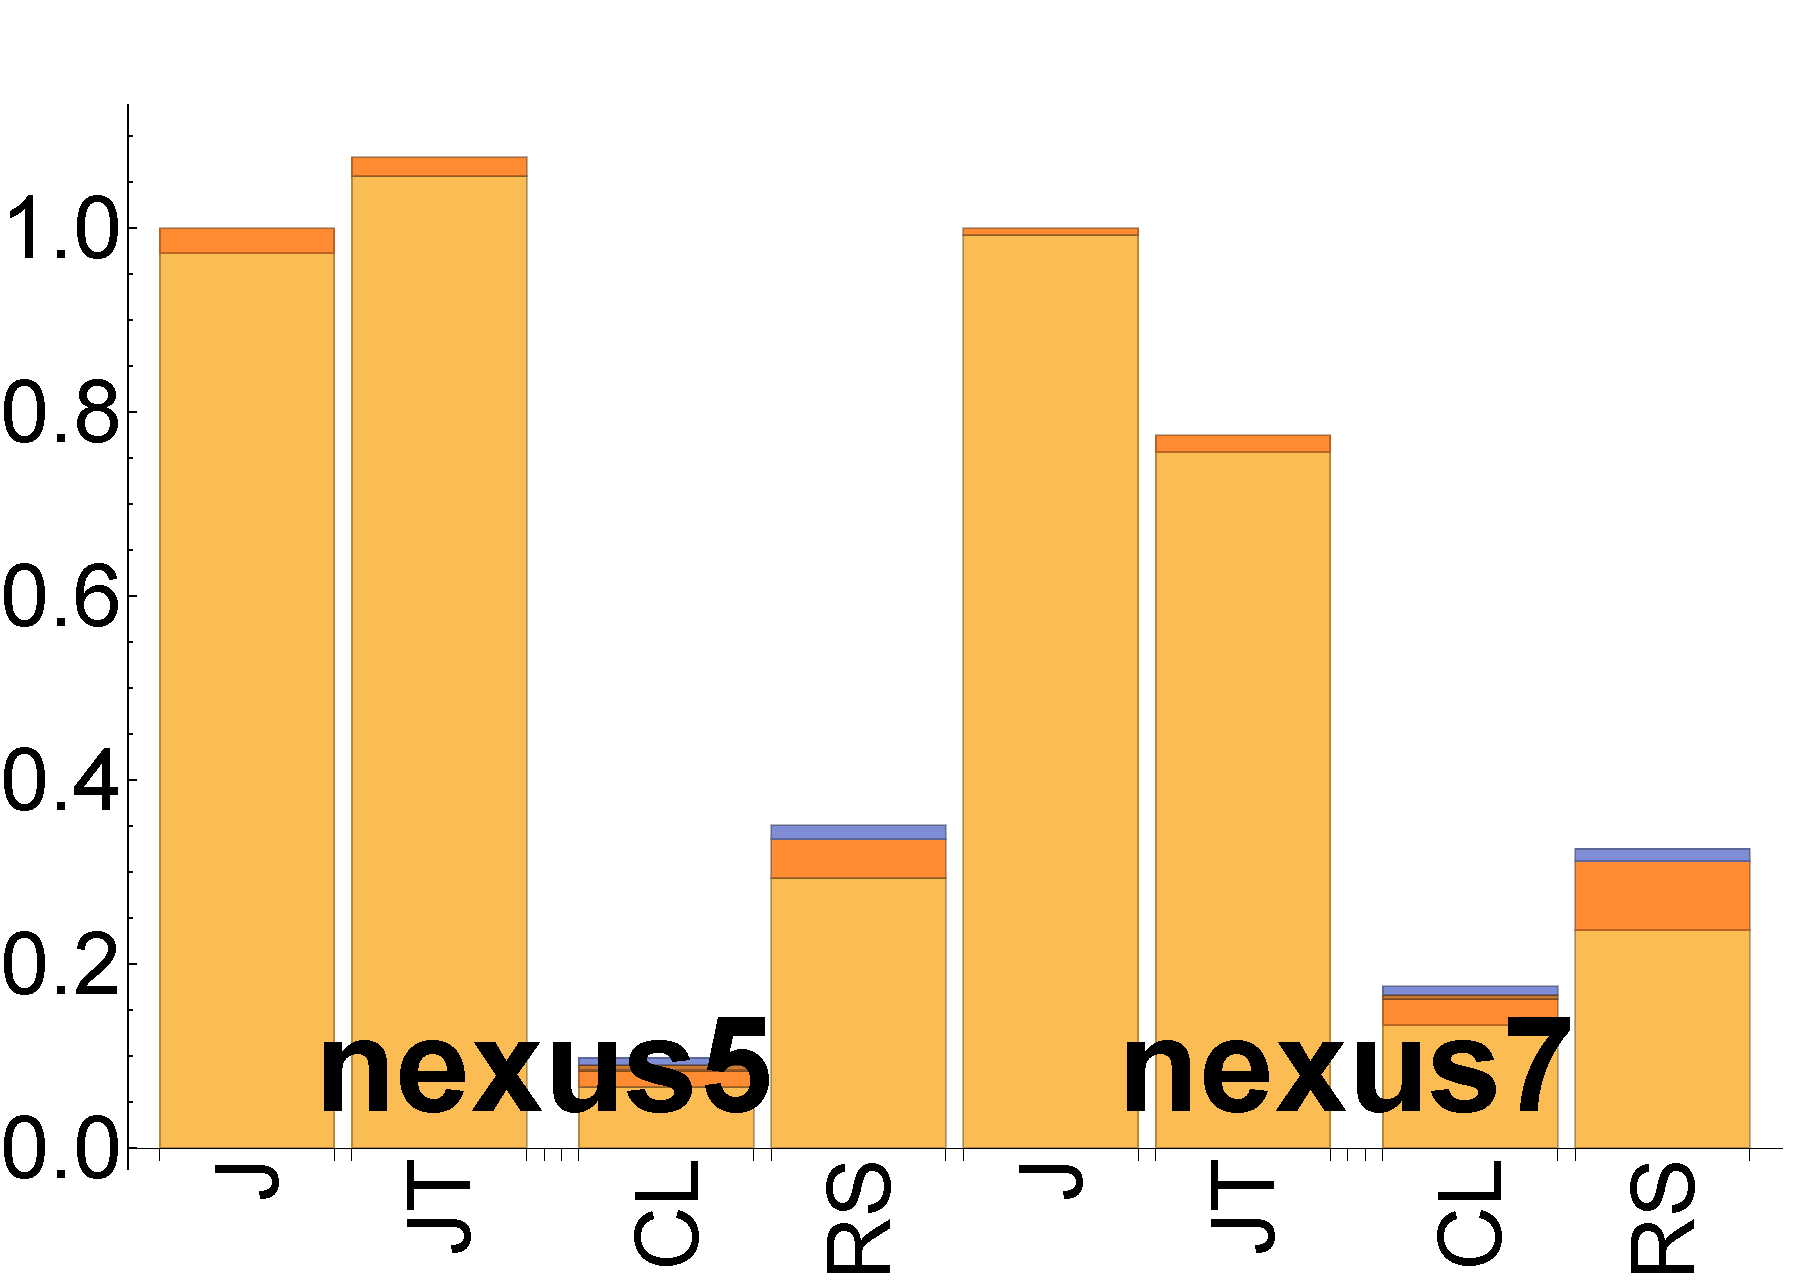
\includegraphics[width=\textwidth]{data/bbattery_tpacf.pdf}
      \caption{TPACF} \label{fig:b_TPACF}
  \end{subfigure}%

  \begin{subfigure}[b]{0.24\textwidth}
      \centering
      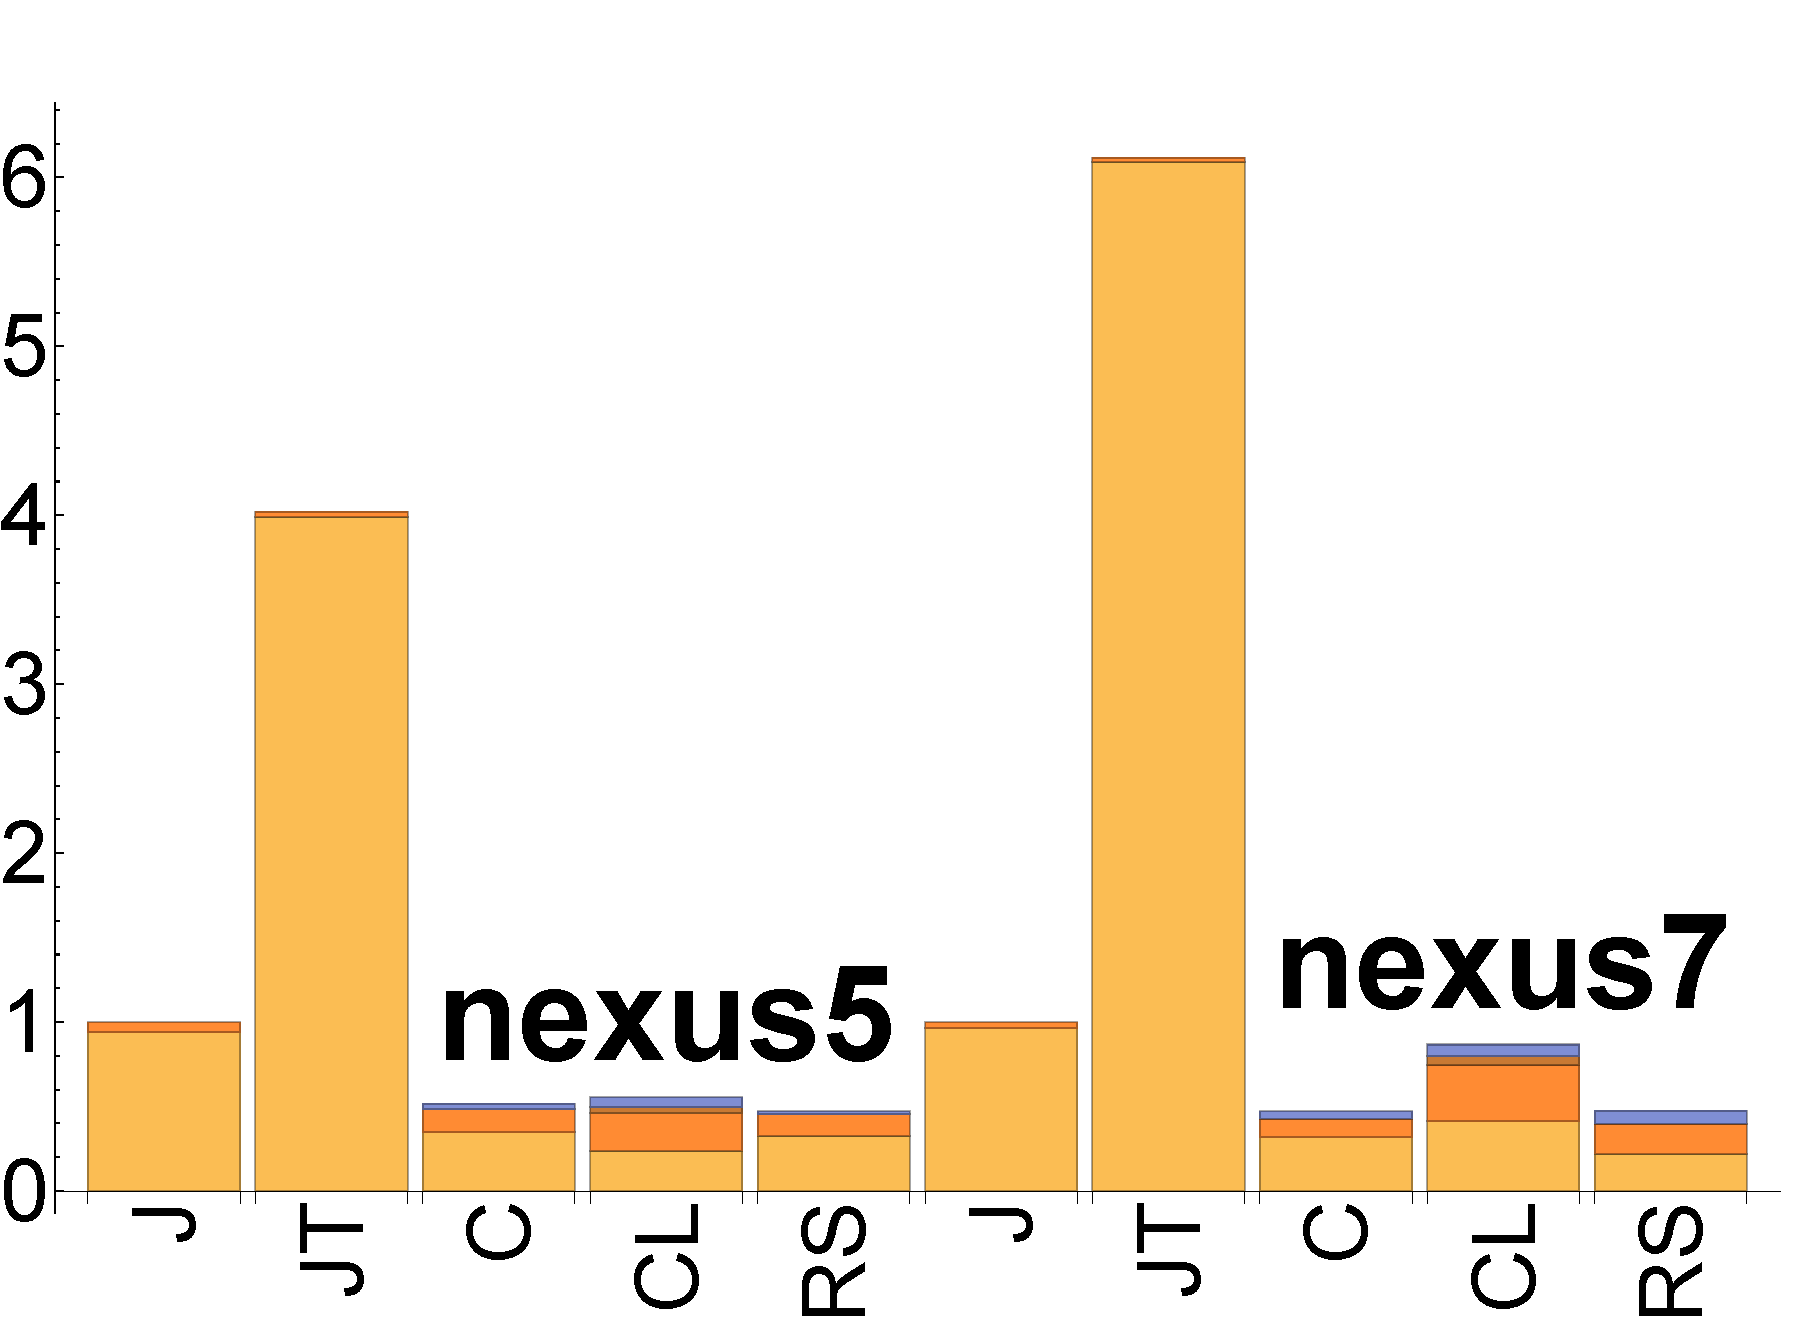
\includegraphics[width=\textwidth]{data/bbattery_histogram.pdf}
      \caption{Histogram}\label{fig:b_histo}
  \end{subfigure}%

  \begin{subfigure}[b]{0.24\textwidth}
      \centering
      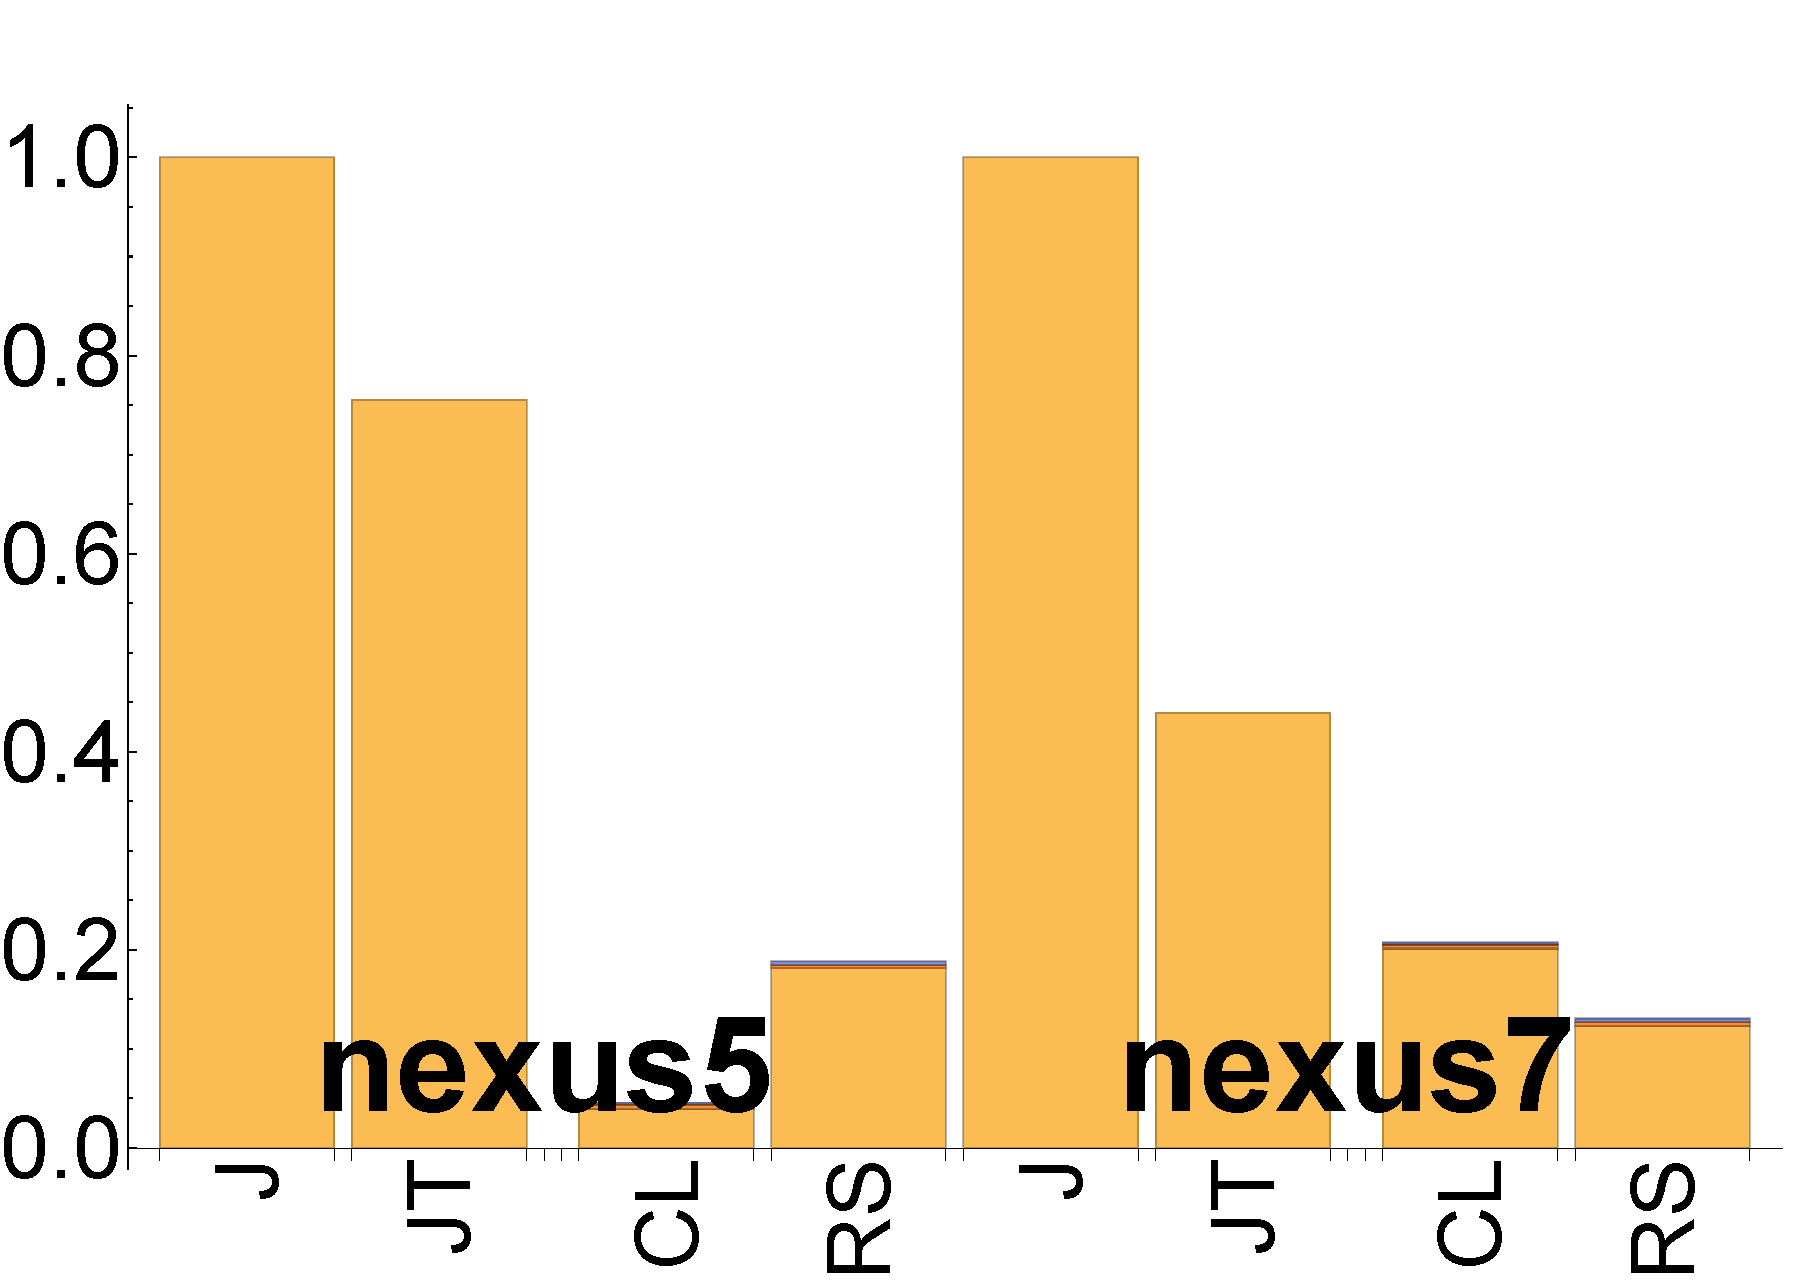
\includegraphics[width=\textwidth]{data/bbattery_mriq.pdf}
      \caption{MRIQ} \label{fig:b_MRIQ}
  \end{subfigure}

  \begin{subfigure}[b]{0.24\textwidth}
      \centering
      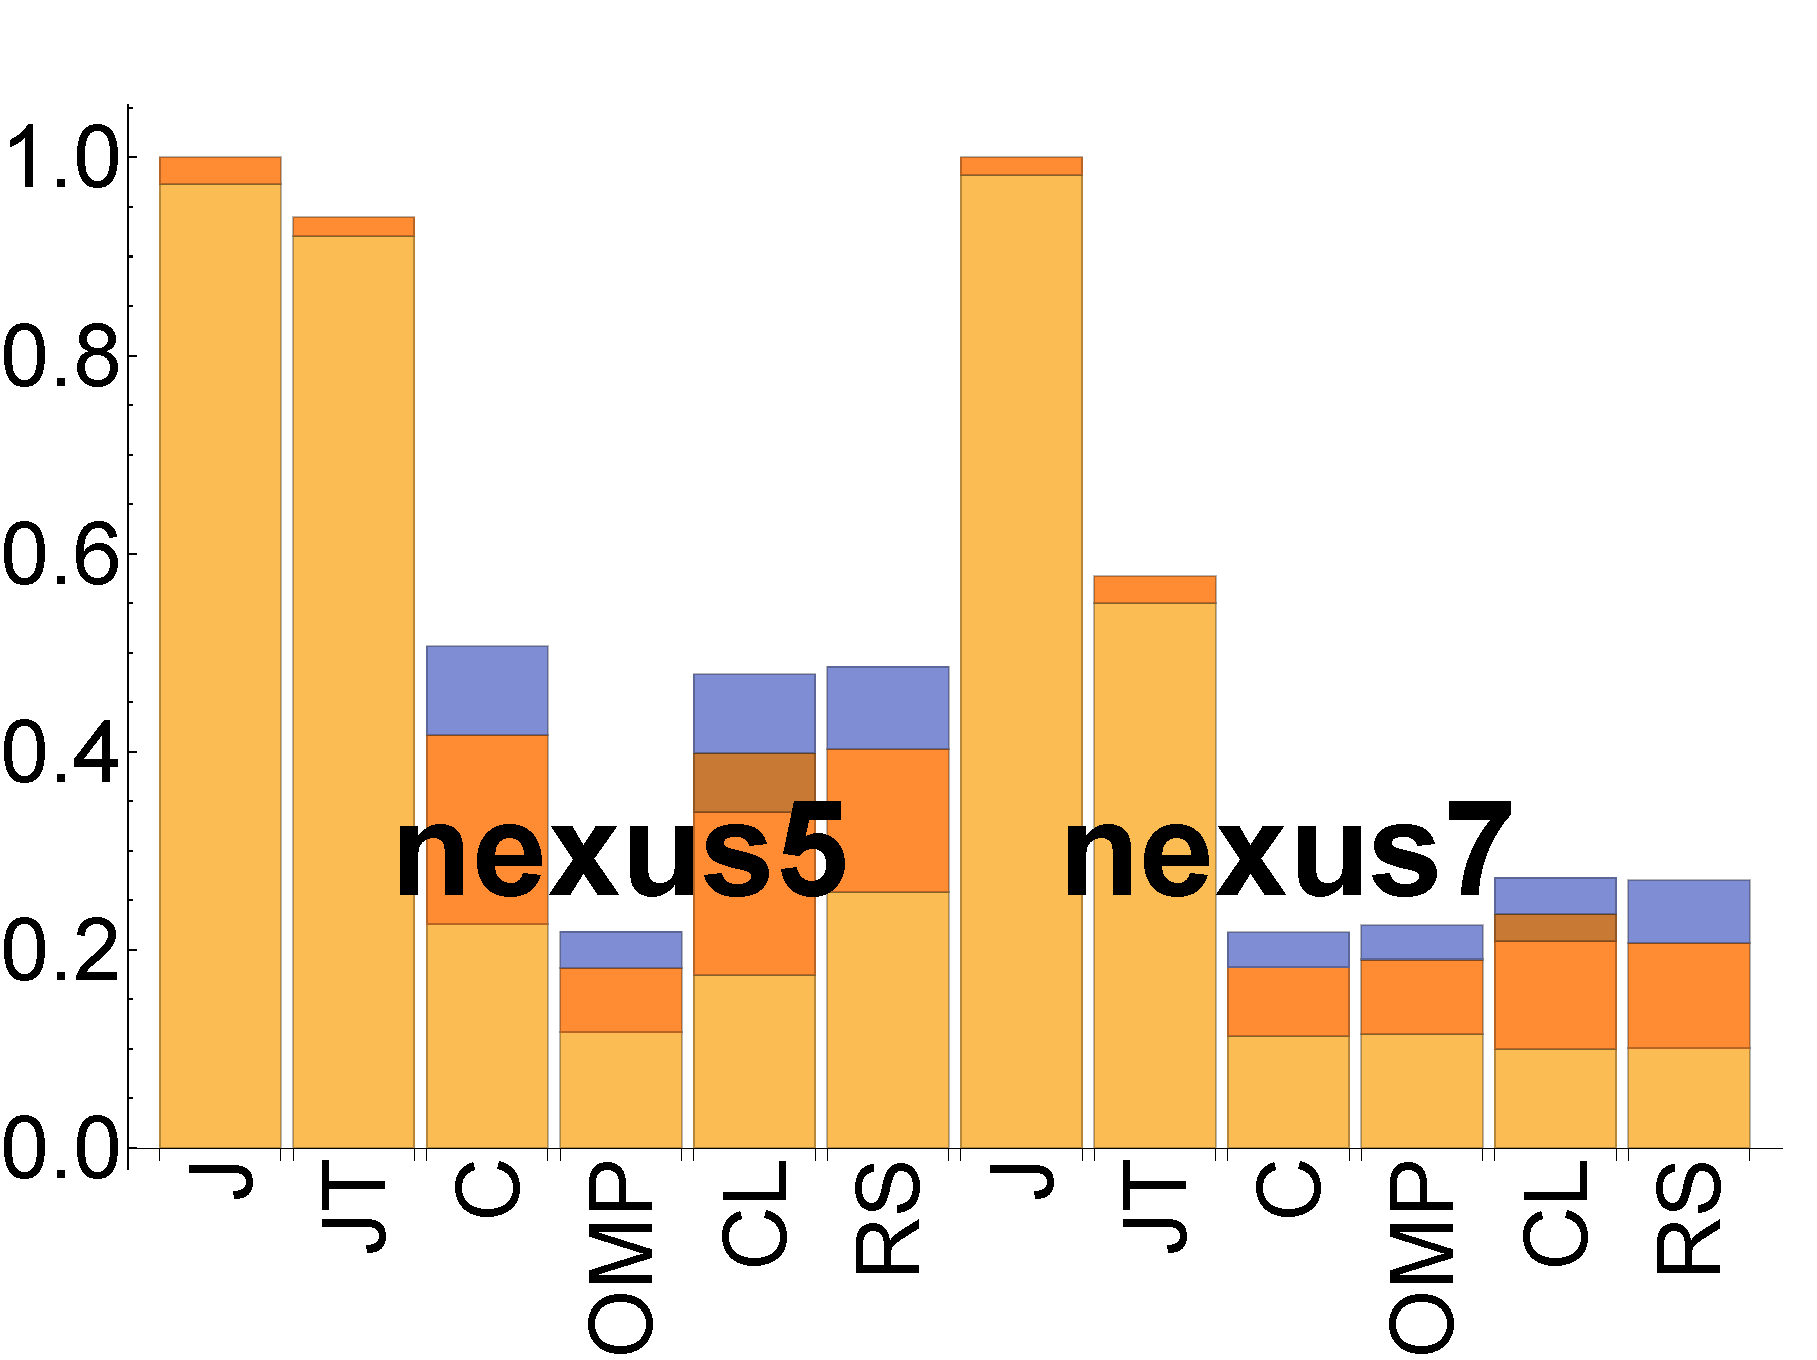
\includegraphics[width=\textwidth]{data/bbattery_sgemm.pdf}
      \caption{Sgemm}\label{fig:b_Sgemm}
  \end{subfigure}

  \begin{subfigure}[b]{0.24\textwidth}
      \centering
      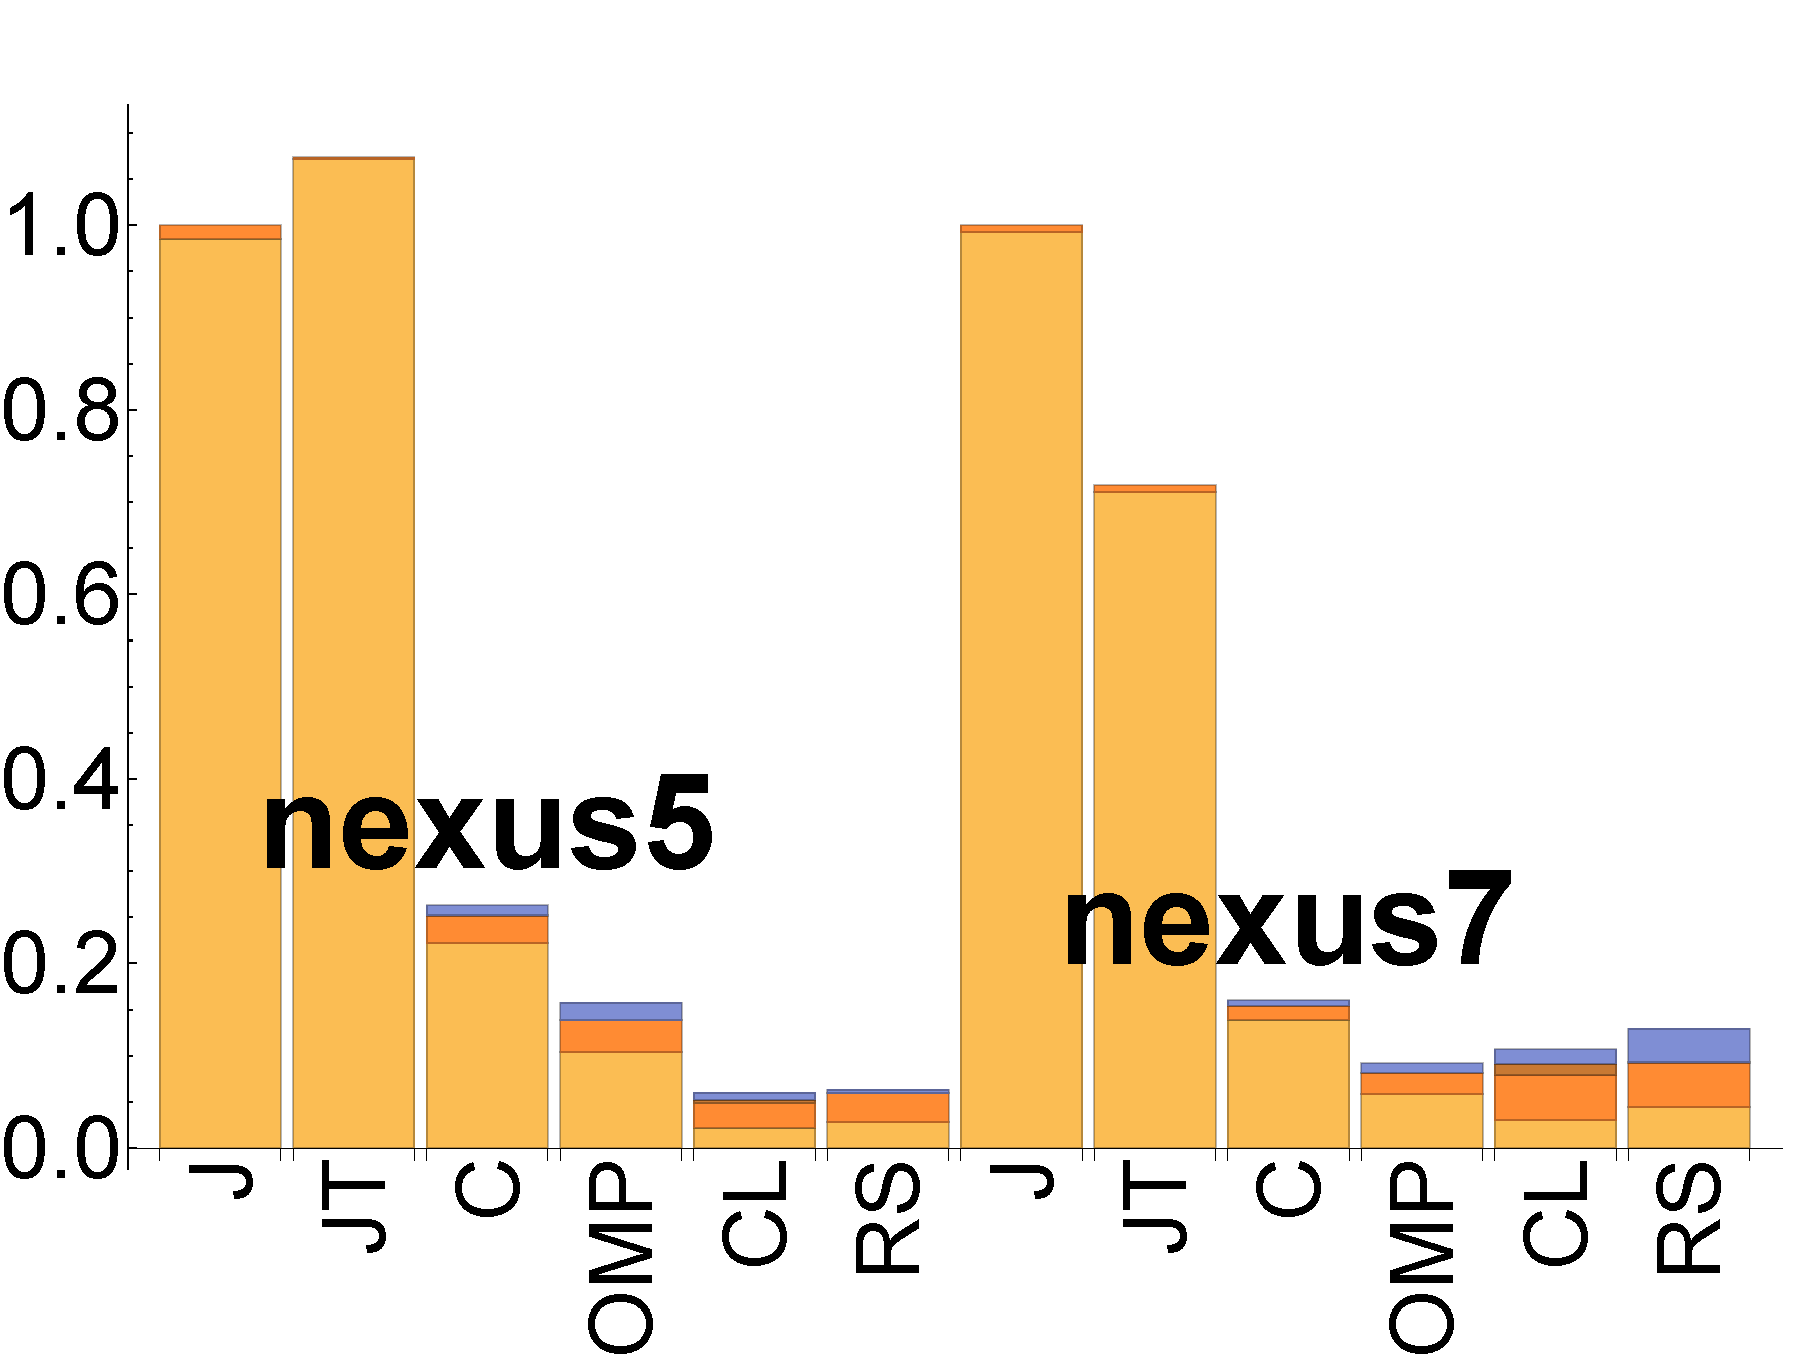
\includegraphics[width=\textwidth]{data/bbattery_stencil.pdf}
      \caption{Stencil} \label{fig:b_Stencil}
  \end{subfigure}

  \caption{Battery Information}
\end{figure}
\FloatBarrier



\subsubsection{Vector Add}

\subsubsection{SGEMM}

\subsubsection{Stencil}

\subsubsection{TPACF}

\subsubsection{MriQ}

\subsubsection{Histogram}

\subsubsection{CUTCP}
